\documentclass[tikz,border=5pt]{standalone}
\begin{document}
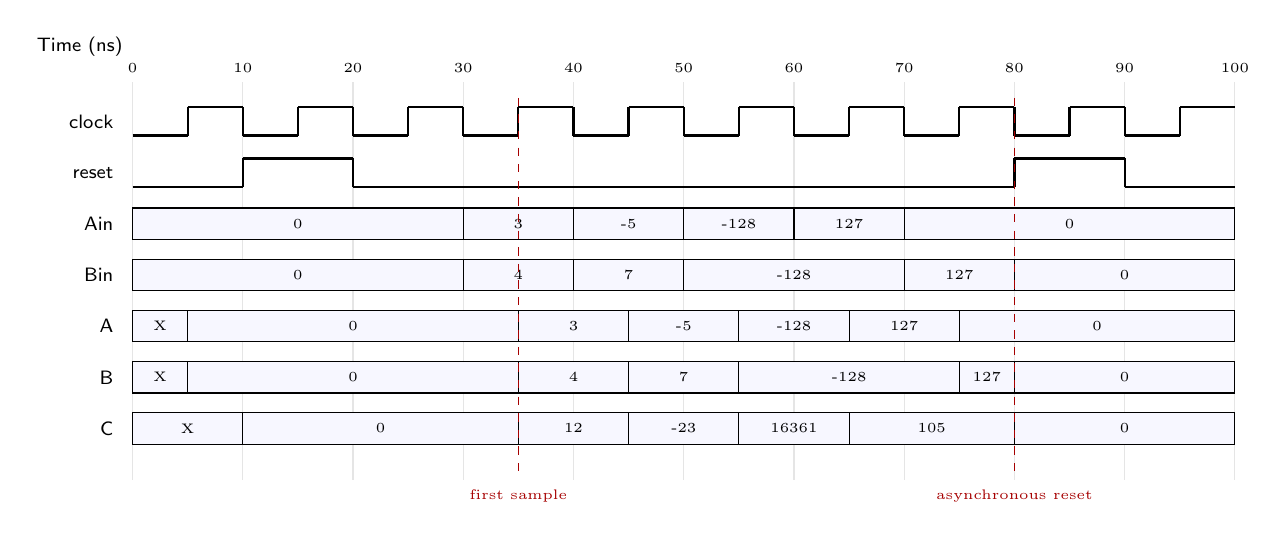
\begin{tikzpicture}[x=1cm,y=1cm,font=\sffamily\scriptsize]
\draw[gray!20] (0.0000,.5)--(0.0000,-4.550);
\node[above,font=\tiny] at (0.0000,.5) {0};
\draw[gray!20] (1.4000,.5)--(1.4000,-4.550);
\node[above,font=\tiny] at (1.4000,.5) {10};
\draw[gray!20] (2.8000,.5)--(2.8000,-4.550);
\node[above,font=\tiny] at (2.8000,.5) {20};
\draw[gray!20] (4.2000,.5)--(4.2000,-4.550);
\node[above,font=\tiny] at (4.2000,.5) {30};
\draw[gray!20] (5.6000,.5)--(5.6000,-4.550);
\node[above,font=\tiny] at (5.6000,.5) {40};
\draw[gray!20] (7.0000,.5)--(7.0000,-4.550);
\node[above,font=\tiny] at (7.0000,.5) {50};
\draw[gray!20] (8.4000,.5)--(8.4000,-4.550);
\node[above,font=\tiny] at (8.4000,.5) {60};
\draw[gray!20] (9.8000,.5)--(9.8000,-4.550);
\node[above,font=\tiny] at (9.8000,.5) {70};
\draw[gray!20] (11.2000,.5)--(11.2000,-4.550);
\node[above,font=\tiny] at (11.2000,.5) {80};
\draw[gray!20] (12.6000,.5)--(12.6000,-4.550);
\node[above,font=\tiny] at (12.6000,.5) {90};
\draw[gray!20] (14.0000,.5)--(14.0000,-4.550);
\node[above,font=\tiny] at (14.0000,.5) {100};
\node[left] at (0,.95) {Time (ns)};
\node[left] at (-.12,0.000) {clock};
\draw[thick] (0.0000,-0.180)--(0.7000,-0.180);
\draw[thick] (0.7000,0.180)--(1.4000,0.180);
\draw[thick] (0.7000,-0.180)--(0.7000,0.180);
\draw[thick] (1.4000,-0.180)--(2.1000,-0.180);
\draw[thick] (1.4000,-0.180)--(1.4000,0.180);
\draw[thick] (2.1000,0.180)--(2.8000,0.180);
\draw[thick] (2.1000,-0.180)--(2.1000,0.180);
\draw[thick] (2.8000,-0.180)--(3.5000,-0.180);
\draw[thick] (2.8000,-0.180)--(2.8000,0.180);
\draw[thick] (3.5000,0.180)--(4.2000,0.180);
\draw[thick] (3.5000,-0.180)--(3.5000,0.180);
\draw[thick] (4.2000,-0.180)--(4.9000,-0.180);
\draw[thick] (4.2000,-0.180)--(4.2000,0.180);
\draw[thick] (4.9000,0.180)--(5.6000,0.180);
\draw[thick] (4.9000,-0.180)--(4.9000,0.180);
\draw[thick] (5.6000,-0.180)--(6.3000,-0.180);
\draw[thick] (5.6000,-0.180)--(5.6000,0.180);
\draw[thick] (6.3000,0.180)--(7.0000,0.180);
\draw[thick] (6.3000,-0.180)--(6.3000,0.180);
\draw[thick] (7.0000,-0.180)--(7.7000,-0.180);
\draw[thick] (7.0000,-0.180)--(7.0000,0.180);
\draw[thick] (7.7000,0.180)--(8.4000,0.180);
\draw[thick] (7.7000,-0.180)--(7.7000,0.180);
\draw[thick] (8.4000,-0.180)--(9.1000,-0.180);
\draw[thick] (8.4000,-0.180)--(8.4000,0.180);
\draw[thick] (9.1000,0.180)--(9.8000,0.180);
\draw[thick] (9.1000,-0.180)--(9.1000,0.180);
\draw[thick] (9.8000,-0.180)--(10.5000,-0.180);
\draw[thick] (9.8000,-0.180)--(9.8000,0.180);
\draw[thick] (10.5000,0.180)--(11.2000,0.180);
\draw[thick] (10.5000,-0.180)--(10.5000,0.180);
\draw[thick] (11.2000,-0.180)--(11.9000,-0.180);
\draw[thick] (11.2000,-0.180)--(11.2000,0.180);
\draw[thick] (11.9000,0.180)--(12.6000,0.180);
\draw[thick] (11.9000,-0.180)--(11.9000,0.180);
\draw[thick] (12.6000,-0.180)--(13.3000,-0.180);
\draw[thick] (12.6000,-0.180)--(12.6000,0.180);
\draw[thick] (13.3000,0.180)--(14.0000,0.180);
\draw[thick] (13.3000,-0.180)--(13.3000,0.180);
\node[left] at (-.12,-0.650) {reset};
\draw[thick] (0.0000,-0.830)--(1.4000,-0.830);
\draw[thick] (1.4000,-0.470)--(2.8000,-0.470);
\draw[thick] (1.4000,-0.830)--(1.4000,-0.470);
\draw[thick] (2.8000,-0.830)--(11.2000,-0.830);
\draw[thick] (2.8000,-0.830)--(2.8000,-0.470);
\draw[thick] (11.2000,-0.470)--(12.6000,-0.470);
\draw[thick] (11.2000,-0.830)--(11.2000,-0.470);
\draw[thick] (12.6000,-0.830)--(14.0000,-0.830);
\draw[thick] (12.6000,-0.830)--(12.6000,-0.470);
\node[left] at (-.12,-1.300) {Ain};
\draw[fill=blue!3] (0.0000,-1.500) rectangle (4.2000,-1.100);
\node[font=\tiny] at (2.1000,-1.300) {0};
\draw[fill=blue!3] (4.2000,-1.500) rectangle (5.6000,-1.100);
\node[font=\tiny] at (4.9000,-1.300) {3};
\draw[fill=blue!3] (5.6000,-1.500) rectangle (7.0000,-1.100);
\node[font=\tiny] at (6.3000,-1.300) {-5};
\draw[fill=blue!3] (7.0000,-1.500) rectangle (8.4000,-1.100);
\node[font=\tiny] at (7.7000,-1.300) {-128};
\draw[fill=blue!3] (8.4000,-1.500) rectangle (9.8000,-1.100);
\node[font=\tiny] at (9.1000,-1.300) {127};
\draw[fill=blue!3] (9.8000,-1.500) rectangle (14.0000,-1.100);
\node[font=\tiny] at (11.9000,-1.300) {0};
\node[left] at (-.12,-1.950) {Bin};
\draw[fill=blue!3] (0.0000,-2.150) rectangle (4.2000,-1.750);
\node[font=\tiny] at (2.1000,-1.950) {0};
\draw[fill=blue!3] (4.2000,-2.150) rectangle (5.6000,-1.750);
\node[font=\tiny] at (4.9000,-1.950) {4};
\draw[fill=blue!3] (5.6000,-2.150) rectangle (7.0000,-1.750);
\node[font=\tiny] at (6.3000,-1.950) {7};
\draw[fill=blue!3] (7.0000,-2.150) rectangle (9.8000,-1.750);
\node[font=\tiny] at (8.4000,-1.950) {-128};
\draw[fill=blue!3] (9.8000,-2.150) rectangle (11.2000,-1.750);
\node[font=\tiny] at (10.5000,-1.950) {127};
\draw[fill=blue!3] (11.2000,-2.150) rectangle (14.0000,-1.750);
\node[font=\tiny] at (12.6000,-1.950) {0};
\node[left] at (-.12,-2.600) {A};
\draw[fill=blue!3] (0.0000,-2.800) rectangle (0.7000,-2.400);
\node[font=\tiny] at (0.3500,-2.600) {X};
\draw[fill=blue!3] (0.7000,-2.800) rectangle (4.9000,-2.400);
\node[font=\tiny] at (2.8000,-2.600) {0};
\draw[fill=blue!3] (4.9000,-2.800) rectangle (6.3000,-2.400);
\node[font=\tiny] at (5.6000,-2.600) {3};
\draw[fill=blue!3] (6.3000,-2.800) rectangle (7.7000,-2.400);
\node[font=\tiny] at (7.0000,-2.600) {-5};
\draw[fill=blue!3] (7.7000,-2.800) rectangle (9.1000,-2.400);
\node[font=\tiny] at (8.4000,-2.600) {-128};
\draw[fill=blue!3] (9.1000,-2.800) rectangle (10.5000,-2.400);
\node[font=\tiny] at (9.8000,-2.600) {127};
\draw[fill=blue!3] (10.5000,-2.800) rectangle (14.0000,-2.400);
\node[font=\tiny] at (12.2500,-2.600) {0};
\node[left] at (-.12,-3.250) {B};
\draw[fill=blue!3] (0.0000,-3.450) rectangle (0.7000,-3.050);
\node[font=\tiny] at (0.3500,-3.250) {X};
\draw[fill=blue!3] (0.7000,-3.450) rectangle (4.9000,-3.050);
\node[font=\tiny] at (2.8000,-3.250) {0};
\draw[fill=blue!3] (4.9000,-3.450) rectangle (6.3000,-3.050);
\node[font=\tiny] at (5.6000,-3.250) {4};
\draw[fill=blue!3] (6.3000,-3.450) rectangle (7.7000,-3.050);
\node[font=\tiny] at (7.0000,-3.250) {7};
\draw[fill=blue!3] (7.7000,-3.450) rectangle (10.5000,-3.050);
\node[font=\tiny] at (9.1000,-3.250) {-128};
\draw[fill=blue!3] (10.5000,-3.450) rectangle (11.2000,-3.050);
\node[font=\tiny] at (10.8500,-3.250) {127};
\draw[fill=blue!3] (11.2000,-3.450) rectangle (14.0000,-3.050);
\node[font=\tiny] at (12.6000,-3.250) {0};
\node[left] at (-.12,-3.900) {C};
\draw[fill=blue!3] (0.0000,-4.100) rectangle (1.4000,-3.700);
\node[font=\tiny] at (0.7000,-3.900) {X};
\draw[fill=blue!3] (1.4000,-4.100) rectangle (4.9000,-3.700);
\node[font=\tiny] at (3.1500,-3.900) {0};
\draw[fill=blue!3] (4.9000,-4.100) rectangle (6.3000,-3.700);
\node[font=\tiny] at (5.6000,-3.900) {12};
\draw[fill=blue!3] (6.3000,-4.100) rectangle (7.7000,-3.700);
\node[font=\tiny] at (7.0000,-3.900) {-23};
\draw[fill=blue!3] (7.7000,-4.100) rectangle (9.1000,-3.700);
\node[font=\tiny] at (8.4000,-3.900) {16361};
\draw[fill=blue!3] (9.1000,-4.100) rectangle (11.2000,-3.700);
\node[font=\tiny] at (10.1500,-3.900) {105};
\draw[fill=blue!3] (11.2000,-4.100) rectangle (14.0000,-3.700);
\node[font=\tiny] at (12.6000,-3.900) {0};
\draw[red!65!black,dashed] (4.9000,.3)--(4.9000,-4.550);
\node[below,font=\tiny,text=red!65!black] at (4.9000,-4.550) {first sample};
\draw[red!65!black,dashed] (11.2000,.3)--(11.2000,-4.550);
\node[below,font=\tiny,text=red!65!black] at (11.2000,-4.550) {asynchronous reset};
\end{tikzpicture}
\end{document}
